\begin{figure}[htbp]
  \centering
  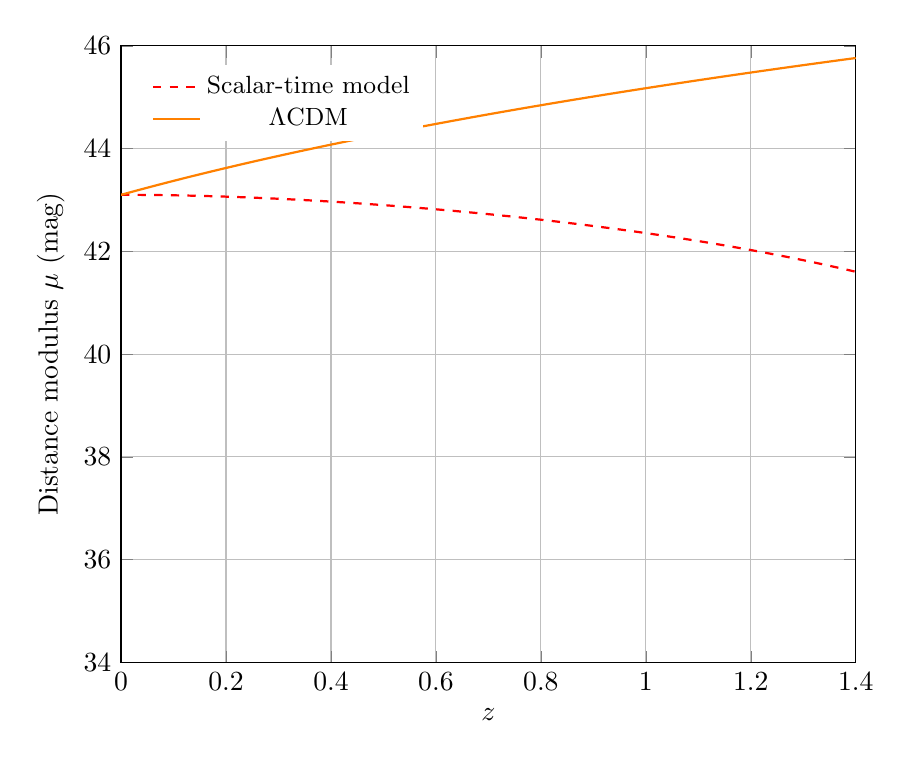
\begin{tikzpicture}
  \begin{axis}[
      width=0.9\textwidth,
      xlabel={$z$},
      ylabel={Distance modulus $\mu$ (mag)},
      xmin=0, xmax=1.4,
      ymin=34, ymax=46,
      grid=both,
      legend style={draw=none, font=\small},
      legend pos=north west]
    % scalar-time (toy) curve
    \addplot[red,dashed,thick,domain=0:1.4,samples=150]
      {43.1 + 5*log10((1+x)*((1-0.45*x)/(1+0.55*x)))};
    \addlegendentry{Scalar-time model}
    % ΛCDM comparison curve
    \addplot[orange,thick,domain=0:1.4,samples=150]
      {43.1 + 5*log10((1+x)*(1+0.3*x))};
    \addlegendentry{$\Lambda$CDM}
  \end{axis}
  \end{tikzpicture}
  %-------------------------------------------------------------
  \caption{Distance–modulus curves for the scalar-time model (red dashed) and a reference $\Lambda$CDM fit (orange). Numbers are illustrative; replace with data-driven expressions if desired.}
  \label{fig:DistModulus}
\end{figure}
